\documentclass[10pt]{beamer}

\usepackage{beamerthemesplit}
\usepackage{graphics}
\usepackage{amssymb,amsmath}
\usepackage{verbatim}
\usepackage{hyperref}
\usepackage{multirow}
\usepackage{array}

\usepackage{pifont}% http://ctan.org/pkg/pifont
\newcommand{\cmark}{\ding{51}}%
\newcommand{\xmark}{\ding{55}}%

%\setcounter{MaxMatrixCols}{30}

\newtheorem{thm}{Theorem}[section]
\newtheorem{SmithQuote}[thm]{Quote}
\newtheorem{srp}[thm]{Surprise!}
\newtheorem{lem}[thm]{Lemma}
\newtheorem{prop}[thm]{Proposition}
\newtheorem{cor}[thm]{Corollary}
\theoremstyle{definition}
\newtheorem{defn}{Definition}[section]
\newtheorem{ntn}{Notation}[section]
\newtheorem{properties}[thm]{Properties}
\theoremstyle{remark}
\newtheorem{rmk}{Remark}[section]
\newtheorem{eg}{Example}[section]
\newtheorem{conc}{Conlusion}[section]
\newtheorem{qn}{Question}[section]
\newtheorem{hth}{Hypothesis}[section]
\newtheorem{conj}{Conjecture}[section]

%Mathmode shortcuts
\newcommand{\TextNorm}[1]{\textrm{\textmd{\textup{#1}}}}
\newcommand{\hsforall}{\hspace{1mm}\forall\hspace{1mm}}						 %Spacing around \forall
\newcommand{\hsexists}{\hspace{1mm}\exists\hspace{1mm}} 					 %Spacing around \exists
\newcommand{\Mspacer}{\hspace{0.5mm}}                              %Spacer for below Matrix display functions
\newcommand{\M}[3]{#1_{#2\Mspacer#3}}                              %Print a symbol with two subscripts eg a matrix entry
\newcommand{\Msup}[4]{#1_{#2\Mspacer#3}^{#4}}                      %Print a symbol with two subscripts and a superscript eg a matrix entry
\newcommand{\Msups}[5]{#1_{#2\Mspacer#3}^{#4\Mspacer#5}}           %Print a symbol with two subscripts and two superscripts eg a matrix entry
\newcommand{\Trace}{\text{\TextNorm{Tr}}\hspace{0.5mm}}            %Trace of something, eg a contour
\newcommand{\res}{\operatorname*{Res}}                             %Residue of an expression
\newcommand{\PV}{\text{\TextNorm{PV}}\hspace{0.5mm}}               %Principal Value of an integral
\renewcommand{\Re}{\operatorname*{Re}}                             %Real part of something
\renewcommand{\Im}{\operatorname*{Im}}                             %Imaginary part of something
\newcommand{\dist}{\text{\TextNorm{dist}}\hspace{0.5mm}}					 %dist function
\renewcommand{\D}{\text{\TextNorm{d}}\hspace{0.1mm}}							 %an upright d for infintessimals
\newcommand{\sgn}{\text{\TextNorm{sgn}}\hspace{0.5mm}}						 %Sign of a real number or permutation
\newcommand{\DeltaP}{\Delta_{\text{\TextNorm{PDE}}}\hspace{0.5mm}} %Sign of a real number or permutation
%\newcommand{\DeltaPstar}{\Delta_{\mathrm{PDE}}^\star\hspace{0.5mm}}%The function whose zeros form the adjoint PDE discrete spectrum
%\newcommand{\M}[3]{#1_{#2\hspace{0.5mm}#3}}                        %Print a symbol with two subscripts eg a matrix entry
%\renewcommand{\geq}{\geqslant}                                     %Always use \geqslant, never the standard \geq
%\renewcommand{\leq}{\leqslant}                                     %Always use \leqslant, never the standard \leq
%\newcommand{\BE}{\begin{equation}}                                 %Begin an equation environment
%\newcommand{\EE}{\end{equation}}                                   %End an equation environment
%\newcommand{\BES}{\begin{equation*}}                               %Begin an equation* environment
%\newcommand{\EES}{\end{equation*}}                                 %End an equation* environment
\newcommand{\BP}{\begin{pmatrix}}                                  %Begin a pmatrix environment
\newcommand{\EP}{\end{pmatrix}}                                    %End a pmatrix environment
%\newcommand{\Iff}{\ensuremath{\Leftrightarrow}}                    %Shorthand for bidirectional implication
\newcommand{\N}{\mathbb{N}}                                        %Shorthand for the set of natural numbers
\newcommand{\Z}{\mathbb{Z}}                                        %Shorthand for the set of integers
\newcommand{\Q}{\mathbb{Q}}                                        %Shorthand for the set of rational numbers
\newcommand{\R}{\mathbb{R}}                                        %Shorthand for the set of real numbers
\newcommand{\C}{\mathbb{C}}                                        %Shorthand for the set of complex numbers

%Superscripts in text
\newcommand{\superscript}[1]{\ensuremath{^{\textrm{#1}}}}
\newcommand{\subscript}[1]{\ensuremath{_{\textrm{#1}}}}
\newcommand{\Thns}[0]{\superscript{th}}
\newcommand{\Th}[0]{\Thns~}
\newcommand{\stns}[0]{\superscript{st}}
\newcommand{\st}[0]{\stns~}
\newcommand{\ndns}[0]{\superscript{nd}}
\newcommand{\nd}[0]{\ndns~}
\newcommand{\rdns}[0]{\superscript{rd}}
\newcommand{\rd}[0]{\rdns~}


\usetheme{Boadilla}

\definecolor{dark-blue}{rgb}{0,0,0.5}
\definecolor{dark-green}{rgb}{0,0.5,0}
\definecolor{dark-orange}{rgb}{0.5,0.25,0}
\definecolor{light-gray}{rgb}{0.8,0.8,0.8}

\newcommand{\Handout}[1]{{\color{orange}\##1}}

\title[Nonlocal Fokas Method]{Nonlocal problems for linear evolution equations}
\author[DA Smith]{Dave Smith}
\institute[Math, Yale-NUS]{Yale-NUS College}
\date[2019-05-22]{University of California Santa Cruz\\Geometry \& Analysis Seminar May 22 2019}
\subject{Nonlocal Fokas Method}

%\AtBeginSection[]
%{
%  \begin{frame}
%    \frametitle{Outline}
%    \tableofcontents[currentsection]
%  \end{frame}
%}

%\includeonlyframes{slide.IBVP.1,slide.Classical.1,slide.Classical.2,slide.FokasIntTrans.1} %%%%%%%%%%%%%%%%%%%%%%%%%%%%%%%%%%%% INCLUDEONLY COMMAND %%%%%%%%%%%%%%%%%%%%%%%%%%%%%%%%%%%%
%\includeonlyframes{slide.AugEig} %%%%%%%%%%%%%%%%%%%%%%%%%%%%%%%%%%%% INCLUDEONLY COMMAND %%%%%%%%%%%%%%%%%%%%%%%%%%%%%%%%%%%%

%\setbeamercovered{transparent}

\begin{document}


\begin{frame}
	\titlepage
	\begin{center}
		\vspace{-3ex}
		
\includegraphics[width=100pt]{./gfx/YNC-Logo}
		
		%\vspace{2ex}
		%{\small\url{http://www-personal.umich.edu/~daasmith/teaching/handouts.zip}}
	\end{center}
\end{frame}


%Frame 0: Thanks
\begin{frame}[label=slide.Papers]
	\frametitle{Papers}
	
	\noindent
	Peter Miller, S. \emph{The diffusion equation with nonlocal data} J. Math. Anal. Appl. {\bf 466} 2. 1119--1143 (2018) arXiv:1708.00972 \\ ~ \\ ~
	
	\noindent
	Beatrice Pelloni, S. \emph{Nonlocal and multipoint boundary value problems for linear evolution equations} Stud. Appl. Math. {\bf 141} 1. 46--88 (2018) arXiv:1511.07244

\end{frame}

%Frame: Mathematical motivation
\begin{frame}[label=slide.Why]
	\frametitle{Nonlocal problems: mathematical motivation}
		Integrable evolution equations in $2+1$ tend to be nonlocal equations.
		
	\vspace{3ex}
	\visible<2->{
		\noindent
		Aim to study {\only<4->{\color{light-gray}}Non}linear evolution equations in {\only<4->{\color{light-gray}}more than} one spatial dimension with {\only<4->{\color{light-gray}}nonlocal terms}\only<2>{.} \visible<3->{{\only<4->{\color{light-gray}}and} nonlocal ``boundary'' conditions.}
	}
	
	\vspace{3ex}
	\visible<5->{
		\noindent
		Heat equation in $1+1$ d with nonlocal ``boundary'' condition.
		\begin{gather*}
			[\partial_t-\partial_x^2]q(x,t) = 0, \qquad
			q(x,0) = {\only<6->{\color{red}}q_0}(x), \qquad
			q_x(1,t) = {\only<6->{\color{red}}g_1}(t), \\
			\int_0^1 {\only<6->{\color{orange}}K}(x)q(x,t) dx = {\only<6->{\color{red}}g_0}(t),
		\end{gather*}
	}
	
	\visible<6->{
		for $q_0,g_j$ have bounded derivatives, $K$ of bounded variation and, at $0$, nonzero and continuous.
	}
	
	\visible<7->{
		Can we solve this problem\only<7>{?}\visible<8->{ using the Fokas Method?}
	}
	
		\vspace{3ex}
	\visible<9->{
		See also: Deconinck Vasan 2013, Fokas Pelloni 2005, Biondini et.\ al.\ 2019(?).
	}
\end{frame}

%Frame: Boundary / Multipoint / Nonlocal conditions
\begin{frame}[label=slide.Why]
	\frametitle{Boundary / Multipoint / Nonlocal conditions}
	\only<1>{
		\noindent
		Domain
		\phantom{Boundary condition}
		\begin{center}\includegraphics[width=0.8\textwidth]{gfx/BC-MC-NC-01}\end{center}
	}
	\only<2>{
		\noindent
		Boundary condition
		\begin{center}\includegraphics[width=0.8\textwidth]{gfx/BC-MC-NC-02}\end{center}
	}
	\only<3>{
		\noindent
		Coupled boundary condition
		\begin{center}\includegraphics[width=0.8\textwidth]{gfx/BC-MC-NC-03}\end{center}
	}
	\only<4>{
		\noindent
		Multipoint condition
		\begin{center}\includegraphics[width=0.8\textwidth]{gfx/BC-MC-NC-04}\end{center}
	}
	\only<5>{
		\noindent
		Nonlocal condition
		\phantom{Boundary condition}
		\begin{center}\includegraphics[width=0.8\textwidth]{gfx/BC-MC-NC-011}\end{center}
	}
	\only<6>{
		\noindent
		Multipoint condition arises as limit of nonlocal conditions
		\begin{center}\includegraphics[width=0.8\textwidth]{gfx/BC-MC-NC-012}\end{center}
	}
	\only<7>{
		\noindent
		Multipoint condition arises as limit of nonlocal conditions
		\begin{center}\includegraphics[width=0.8\textwidth]{gfx/BC-MC-NC-013}\end{center}
	}
	\only<8>{
		\noindent
		Multipoint condition arises as limit of nonlocal conditions
		\begin{center}\includegraphics[width=0.8\textwidth]{gfx/BC-MC-NC-014}\end{center}
	}
	\only<9>{
		\noindent
		Multipoint condition arises as limit of nonlocal conditions
		\begin{center}\includegraphics[width=0.8\textwidth]{gfx/BC-MC-NC-015}\end{center}
	}
	\only<10>{
		\noindent
		Multipoint condition arises as limit of nonlocal conditions
		\begin{center}\includegraphics[width=0.8\textwidth]{gfx/BC-MC-NC-016}\end{center}
	}
	\only<11>{
		\noindent
		Nonlocal condition arises as limit of multipoint conditions
		\begin{center}\includegraphics[width=0.8\textwidth]{gfx/BC-MC-NC-04}\end{center}
	}
	\only<12>{
		\noindent
		Nonlocal condition arises as limit of multipoint conditions
		\begin{center}\includegraphics[width=0.8\textwidth]{gfx/BC-MC-NC-05}\end{center}
	}
	\only<13>{
		\noindent
		Nonlocal condition arises as limit of multipoint conditions
		\begin{center}\includegraphics[width=0.8\textwidth]{gfx/BC-MC-NC-06}\end{center}
	}
	\only<14>{
		\noindent
		Nonlocal condition arises as limit of multipoint conditions
		\begin{center}\includegraphics[width=0.8\textwidth]{gfx/BC-MC-NC-07}\end{center}
	}
	\only<15>{
		\noindent
		Nonlocal condition arises as limit of multipoint conditions
		\begin{center}\includegraphics[width=0.8\textwidth]{gfx/BC-MC-NC-08}\end{center}
	}
	\only<16>{
		\noindent
		Nonlocal condition arises as limit of multipoint conditions
		\begin{center}\includegraphics[width=0.8\textwidth]{gfx/BC-MC-NC-09}\end{center}
	}
	\only<17>{
		\noindent
		Nonlocal condition arises as limit of multipoint conditions
		\begin{center}\includegraphics[width=0.8\textwidth]{gfx/BC-MC-NC-010}\end{center}
	}
		\vspace{80ex}
\end{frame}

%Frame: Piecewise linear $K$
\begin{frame}[label=slide.Why]
	\frametitle{Piecewise linear $K$}
		\noindent
		Suppose $K=1/a$ on $(0,a)$, and $0$ elsewhere. Study
		\begin{gather*}
			[\partial_t-\partial_x^2]q(x,t) = 0, \qquad
			q(x,0) = q_0(x), \qquad
			q_x(1,t) = g_1(t), \\
			\frac{1}{a}\int_0^a q(x,t) dx = g_0(t).
		\end{gather*}
	\uncover<2->{
		\noindent
		Differentiate nonlocal condition in $t$, and apply PDE:
		$$
			\frac{1}{a}\int_0^a\partial_x^2q(x,t) dx = g'_0(t).
		$$
	}
	\uncover<3->{
		\noindent
		Evaluate integral:
		$$
			q_x(a,t) - q_x(0,t) = a g'_0(t).
		$$
	}
		\vspace{80ex}
\end{frame}

%Frame: Physical motivation
\begin{frame}[label=slide.Why]
	\frametitle{Nonlocal problems: physical motivation}
	\only<1-2,5->{
		\begin{center}\includegraphics[width=0.8\textwidth]{gfx/apparatus-01}\end{center}
	}
	\only<3>{
		\begin{center}
\includegraphics[height=45ex]{./gfx/chemist-happy-1.png}\end{center}
	}
	\only<4>{
		\begin{center}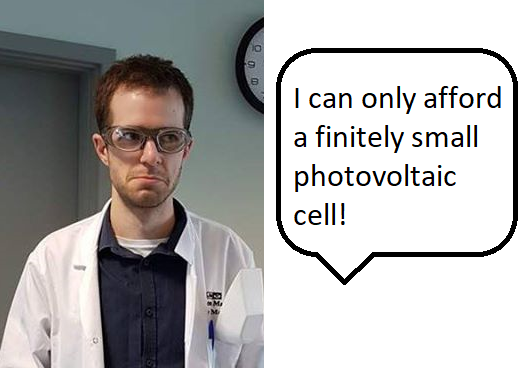
\includegraphics[height=45ex]{./gfx/chemist-sad-1.png}\end{center}
	}
	\only<2>{
		For $q$, concentration of dispersed substance, \\ initial-\emph{boundary} value problem:
		\begin{align*}
			\phantom{K(x)}[\partial_t-\partial_x^2]q(x,t) &= 0 & (x,t) &\in (0,1)\times(0,T),\phantom{K(x)} \\
			q(x,0) &= q_0(x) & x &\in[0,1], \\
			q_x(1,t) &= 0 & t &\in [0,T], \\
			\vphantom{\int_0^1}q(0,t) &= \gamma(t) & t &\in [0,T],
		\end{align*}
	}
	\only<5>{
		For $q$, concentration of dispersed substance, \\ initial-\emph{nonlocal} value problem:
		\begin{align*}
			\phantom{K(x)}[\partial_t-\partial_x^2]q(x,t) &= 0 & (x,t) &\in (0,1)\times(0,T),\phantom{K(x)} \\
			q(x,0) &= q_0(x) & x &\in[0,1], \\
			q_x(1,t) &= 0 & t &\in [0,T], \\
			\vphantom{\int_0^1}\frac{1}{a}\int_0^aq(x,t) dx &= \hat{\gamma}(t) & t &\in [0,T],
		\end{align*}
	}
	\only<6>{
		For $q$, concentration of dispersed substance, \\ initial-\emph{nonlocal} value problem:
		\begin{align*}
			\phantom{K(x)}[\partial_t-\partial_x^2]q(x,t) &= 0 & (x,t) &\in (0,1)\times(0,T),\phantom{K(x)} \\
			q(x,0) &= q_0(x) & x &\in[0,1], \\
			q_x(1,t) &= 0 & t &\in [0,T], \\
			\int_0^1 K(x) q(x,t) dx &= g_0(t) & t &\in [0,T],
		\end{align*}
	}
		\vspace{40ex}
\end{frame}

%Frame 5: FTM.Overview.1
\begin{frame}[label=slide.FTM.Overview.1]
	\frametitle{Overview of Fokas transform method}
	
	\begin{itemize}
		\item{
			Stage 1: assuming existence of a solution, obtain implicit integral representation \& ``global relation''.
		}
		\item{
			Stage 2: continuing from stage 1, obtain explicit integral representation of ``solution'' by implementing \textbf{D}ata\textbf{-to-}u\textbf{N}known map.
			
			Have now established uniqueness of solution.
		}
		\item{
			Stage 3: show that the ``solution'' obtained in stage 2 truly satisfies the problem.
			
			Have now established existence of solution.
		}
	\end{itemize}
	
\end{frame}

%Frame 5: FTM.Overview.1
\begin{frame}[label=slide.FTM.Overview.1]
	\frametitle{Overview of Fokas transform method: Stage 1}
	\begin{enumerate}
		\item[1a]<1-4| only@1-4>{
				Apply Fourier transform $\phi\mapsto\hat{\phi}$, defined by
				$
					\displaystyle \int_{\alt<1>{-\infty\vphantom{y}}{\ooalign{$\hidewidth{\scriptstyle y}\hidewidth$\cr$\phantom{\scriptstyle -\infty}$}}}^{\alt<1>{\infty\vphantom{z}}{\ooalign{$\hidewidth{\scriptstyle \scriptstyle z}\hidewidth$\cr$\phantom{\scriptstyle \infty}$}}}e^{-i\lambda x} \phi(x) dx, \only<2->{\vphantom{\int_{-\infty\vphantom{y}}^{\infty\vphantom{z}}}}
				$
				to PDE:
				$$
					\left[\frac{d}{dt}+\lambda^2\right]\hat{q}(\lambda;t) = \alt<1>{0\phantom{{}-{}e^{-i\lambda y}\big(q_x(y,t) + i\lambda q(y,t)\big) + e^{-i\lambda z}\big(q_x(z,t) + i\lambda q(z,t)\big)}}{ {}-{}e^{-i\lambda y}\big(q_x(y,t) + i\lambda q(y,t)\big) + e^{-i\lambda z}\big(q_x(z,t) + i\lambda q(z,t)\big) \phantom{0}}
				$$
			\only<3-4>{
				Solve the ODE, pretending right side is data, for the \emph{Global relation}:
				\begin{multline*}
					\hat{q}_0(\lambda;y,z) - e^{\lambda^2t}\hat{q}(\lambda;y,z,t) \\
					= e^{-i\lambda y}\left[i\lambda f_0(\lambda;y,t) + f_1(\lambda;y,t)\right]
					- e^{-i\lambda z}\left[i\lambda f_0(\lambda;z,t) + f_1(\lambda;z,t)\right]
				\end{multline*}
				where
				\begin{align*}
					\hat{q}_0(\lambda;y,z) &= \int_y^z e^{-i\lambda x} q_0(x) dx \\
					\hat{q}(\lambda;y,z,t) &= \int_y^z e^{-i\lambda x} q(x,t) dx \\
					f_j(\lambda;y,t) &= \int_0^t e^{\lambda^2s} \partial_x^jq(y,s) ds
				\end{align*}
			}
		}
		\item[1a]<5-| only@5->{
			Global relation:
			$\hat{q}_0(\lambda;y,z) - e^{\lambda^2t}\hat{q}(\lambda;y,z,t) = $ \\
			~
			$ \qquad e^{-i\lambda y}\left[i\lambda f_0(\lambda;y,t) + f_1(\lambda;y,t)\right] - e^{-i\lambda z}\left[i\lambda f_0(\lambda;z,t) + f_1(\lambda;z,t)\right].
			$
		}
		\item[1b]<5-| only@5->{
			Evaluate global relation at $y=0$, $z=1$. Use inverse Fourier transform
			
			\vspace{-4ex}
			\begin{multline*}
				2\pi q(x,t) = \int_{-\infty}^\infty e^{i\lambda x-\lambda^2t} \hat{q}_0(\lambda;0,1) d\lambda \\
				- \int_{\alt<5>{{\color{black}-\infty}{\color{white}\partial D^+}}{{\color{red}\partial D^+}{\color{white}-\infty}}}^{\alt<5>{\infty}{\color{white}\infty}} e^{i\lambda x-\lambda^2t}\left[i\lambda f_0(\lambda;0,t) + f_1(\lambda;0,t)\right] d\lambda \\
				\alt<5>{{\color{white}-}{\color{black}+}}{{\color{white}+}{\color{black}-}} \int_{\alt<5>{{\color{black}-\infty}{\color{white}\partial D^-}}{{\color{red}\partial D^-}{\color{white}-\infty}}}^{\alt<5>{\infty}{\color{white}\infty}} e^{i\lambda (x-1)-\lambda^2t}\left[i\lambda f_0(\lambda;1,t) + f_1(\lambda;1,t)\right] d\lambda
			\end{multline*}
			
			\visible<6>{
				\begin{minipage}[t]{.35\textwidth}
					Define $D^\pm= \\ \{\lambda\in\C^\pm:\Re(\lambda^2)<0\}$. \\ Deform contours \\ using Jordan's lemma.
				\end{minipage}
				\hfill
				\begin{minipage}[t]{.5\textwidth}
					~
					
					\vspace{-3ex}
					\includegraphics[width=0.7\textwidth]{gfx/ContoursD-01}
					
					\vspace{-8ex}
					~
				\end{minipage}
			}
		}
	\end{enumerate}
	
		\vspace{200ex}
\end{frame}

%Frame 6: FTM.Overview.2.BVP
\begin{frame}[label=slide.FTM.Overview.2.BVP]
	\frametitle{Overview of Fokas transform method: Stage 2 (BVP)}
	\begin{itemize}
		\item{
			Global relation:
			$\hat{q}_0(\lambda;y,z) - e^{\lambda^2t}\hat{q}(\lambda;y,z,t) = $ \\
			~ $ \qquad e^{-i\lambda y}\left[i\lambda {\color{blue}f_0(\lambda;y,t)} + {\color{blue}f_1(\lambda;y,t)}\right] - e^{-i\lambda z}\left[i\lambda {\color{blue}f_0(\lambda;z,t)} + {\color{blue}f_1(\lambda;z,t)}\right]$.
		}
		\item{
			Ehrenpreis form:
			$2\pi q(x,t) = \int_{-\infty}^\infty e^{i\lambda x-\lambda^2t} \hat{q}_0(\lambda;0,1) d\lambda$ \\
			~ $\qquad - \int_{\partial D^+} e^{i\lambda x-\lambda^2t}[i\lambda {\alt<1>{\color{red}}{\color{dark-green}}f_0(\lambda;0,t)} + {\color{red}f_1(\lambda;0,t)}] d\lambda$ \\
			~ $\qquad + \int_{\partial D^-} e^{i\lambda (x-1)-\lambda^2t}[i\lambda {\alt<1>{\color{red}}{\color{dark-green}}f_0(\lambda;1,t)} + {\color{red}f_1(\lambda;1,t)}] d\lambda$.
		}
		\item{
			Definitions:
			$\hat{q}_0(\lambda;y,z) = \int_y^z e^{-i\lambda x} q_0(x) dx$,
			$\hat{q}(\lambda;y,z,t) = \int_y^z e^{-i\lambda x} q(x,t) dx$,
			${\color{blue}f_j(\lambda;y,t) = \int_0^t e^{\lambda^2s} \partial_x^jq(y,s) ds}$.
		}
	\end{itemize}
	\begin{enumerate}
		\item[2a]<2->{
			Dirichlet BC give ${\color{dark-green}f_0(\lambda;0,t)}$ and ${\color{dark-green}f_0(\lambda;1,t)}$ explicitly.
		}
		\item[2b]<3->{
			Use global relation at $y=0$, $z=1$: \\
			$\hat{q}_0(\lambda;0,1) - e^{\lambda^2t}\hat{q}(\lambda;0,1,t) =$ \\
			~ $\qquad\left[i\lambda {\color{dark-green}f_0(\lambda;0,t)} + {\color{red}f_1(\lambda;0,t)}\right]
			- e^{-i\lambda}\left[i\lambda {\color{dark-green}f_0(\lambda;1,t)} + {\color{red}f_1(\lambda;1,t)}\right]$.
				
			\only<4->{
				$\lambda\mapsto-\lambda$ for another linear equation in ${\color{red}f_1(\lambda;0,t)}$ and ${\color{red}f_1(\lambda;1,t)}$.
			}
		}
		\item[2c]<5->{
			Solve linear system, as if $\hat{q}(\lambda;0,1,t)$ is data.
		}
		\item[2d]<6->{
			Substitute into Ehrenpreis form.
		}
		\item[2e]<7->{
			Show terms involving $\hat{q}(\lambda;0,1,t)$ do not contribute to solution representation.
		}
	\end{enumerate}
		\vspace{80ex}
\end{frame}

%Frame 7: FTM.Overview.2.MVP
\begin{frame}[label=slide.FTM.Overview.2.MVP]
	\frametitle{Overview of Fokas transform method: Stage 2 (MVP)}
		For $m\in\N$ consider partition $0=\eta_0<\eta_1<\eta_2<\ldots<\eta_m=1$ and
		two general $(m+1)$-point conditions $k={\only<1>{\color{dark-green}}0},{\only<1>{\color{red}}1}$:
		$$
			\sum_{j=0}^1 \sum_{r=0}^m \Msup{b}{j}{k}{r} \partial_x^j q(\eta_r,t) = g_k(t).
		$$
	\only<1>{
		\begin{center}\includegraphics[width=0.4\textwidth]{gfx/MC-01}\end{center}
	}
	\begin{enumerate}
		\item[2a]<2->{
			time-transform multipoint conditions, $k=0,1$:
			$$
				\sum_{j=0}^1 \sum_{r=0}^m \Msup{b}{j}{k}{r} f_j(\lambda;\eta_r,t) = \int_0^te^{\lambda^2s}g_k(s)ds =: \tilde{g}_k(\lambda;t).
			$$
		}
		\item[2b]<3->{
			Evaluate $y=\eta_r$, $z=\eta_{r+1}$, use $\lambda\mapsto-\lambda$; obtain $2m$ global relations.
			\only<3>{\begin{center}\includegraphics[width=0.4\textwidth]{gfx/MC-02}\hspace{6em}~\end{center}}
		}
		\item[2c]<4->{
			Solve system of $2m+2$ equations in $2m+2$ unknowns:
			$
				f_j(\lambda;\eta_r,t), \qquad r=0,1,\ldots,m,
			$
			as if $\hat{q}(\lambda;\eta_r,\eta_{r+1},t)$ is data.
		}
		\item[2d]<5->{
			Substitute into Ehrenpreis form.
		}
		\item[2e]<6->{
			Show terms involving $\hat{q}(\lambda;\eta_r,\eta_{r+1},t)$ do not contribute to solution representation.
		}
	\end{enumerate}
		\vspace{80ex}
\end{frame}

%Frame: FTM.Overview.2.MVP - expanding upon 2c
\begin{frame}[label=slide.FTM.Overview.2.MVP]
	\frametitle{Stage 2c (MVP): more details}

	\only<1>{
		{\def\sclnga{0.35}\def\sclngb{0.7}}
		Linear system for Multipoint value problem:
		
		$X'\mathcal{B}=\mathcal{Y}+Y$ where
		
		$
			\displaystyle
			X'=\Big(\overbrace{f_0(\lambda;\eta_r),\ldots,f_{n-1}(\lambda;\eta_r)}^{r=0,1,\ldots,m}\Big),
		$
		
		{\footnotesize
		$
			\displaystyle
			Y=\Big(\tilde{g}_0(\lambda),\ldots,\tilde{g}_{n-1}(\lambda),\overbrace{-\hat{q}_0(\lambda;\eta_{r-1},\eta_r),-\hat{q}_0(\alpha\lambda;\eta_{r-1},\eta_r),\ldots,-\hat{q}_0(\alpha^{n-1}\lambda;\eta_{r-1},\eta_r)}^{r=1,2,\ldots,m}\Big),
		$
		}
		
		{\footnotesize
		$
			\displaystyle
			\mathcal{Y}=e^{\lambda^2 t}\Big(0,\ldots,0,\overbrace{\hat{q}(\lambda;\eta_{r-1},\eta_r,t),\hat{q}(\alpha\lambda;\eta_{r-1},\eta_r,t),\ldots,\hat{q}(\alpha^{n-1}\lambda;\eta_{r-1},\eta_r,t)}^{r=1,2,\ldots,m}\Big),
		$
		}
		
		$\displaystyle
			\mathcal{B} &=
			\begin{pmatrix}
				\mathfrak{b}^0 & -e_0 &    0 & \cdots &   0     &   0 \\
				\mathfrak{b}^1 &  e_1 & -e_1 & \cdots &   0     &   0 \\
				\mathfrak{b}^2 &    0 &  e_2 & \cdots &   0     &   0 \\
				\vdots & \vdots & \vdots & \ddots & \vdots & \vdots \\
				\mathfrak{b}^{m-1}& 0 &    0 & \cdots & e_{m-1} & -e_{m-1} \\
				\mathfrak{b}^m &    0 &    0 & \cdots &   0     &  e_m
			\end{pmatrix},
		$
		
		in which
		
		$\mathfrak{b}^r$ is a full $n\times n$ matrix of monomials in $\lambda^{-1}$ encoding the multipoint conditions,
		
		$e_r$ is a full $n\times n$ matrix of exponentials.
	}
	\only<2>{
		Rewrite the MVP system as
		
		$X\mathcal{A}=\mathcal{Y}+Y$ where
		
		entries in $X$ are linear combinations of entries in $X'$,
		
		$\displaystyle
			\mathcal{A} &=
			\begin{pmatrix}
				\beta^0     & -I &  0 & \cdots & 0 & 0 \\
				\beta^1     &  I & -I & \cdots & 0 & 0 \\
				\beta^2     &  0 &  I & \cdots & 0 & 0 \\
				\vdots & \vdots & \vdots & \ddots & \vdots & \vdots \\
				\beta^{m-1} &  0 &  0 & \cdots & I & -I \\
				\beta^m     &  0 &  0 & \cdots & 0 & I
			\end{pmatrix},
		$
		
		in which
		
		$\beta^r$ is a full $n\times n$ matrix of polynomials in $\lambda^{-1}$ encoding the multipoint conditions,
		
		$I$ is the $n\times n$ identity matrix.
		
		\vspace{1ex}
		This system can be solved by hand for general $m$.
	}
	\only<3>{
		Solving by hand, we obtain a Riemann Sum.
		
		\vspace{3ex}
		Under continuum limit $m\to\infty$, obtain an integral.
		
		\vspace{3ex}
		So we have solved the full Nonlocal Problem too \dots
	}
	\only<4>{
		\begin{center}
\includegraphics[height=45ex]{./gfx/chemist-happy-2.png}\end{center}
	}
	\only<5>{
		\begin{center}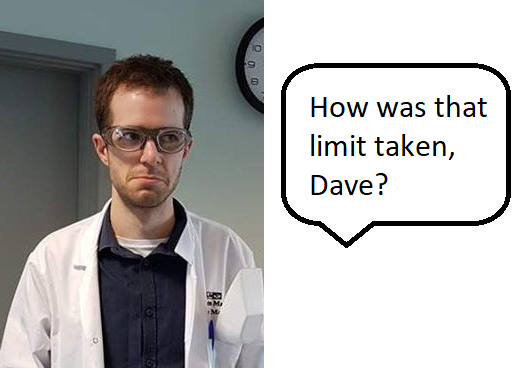
\includegraphics[height=45ex]{./gfx/chemist-sad-3.png}\end{center}
	}
	\only<6->{
		Solving by hand, we obtain a Riemann Sum.
		
		\vspace{3ex}
		Under continuum limit $m\to\infty$, obtain an integral.
		
		\vspace{3ex}
		So we have solved the full Nonlocal Problem too by cheating!
		
		\vspace{3ex}
	}
	\visible<7->{
		We can still implement stage 3 to establish existence \& validity of solution representation, but how do we show uniqueness?
		
		\vspace{3ex}
		Deckert \& Maple 1963 show uniqueness in the case that $K$ is constant.
		
		\vspace{3ex}
		Try to generalise Deckert \& Maple 1963. Difficult.
	}
		\vspace{80ex}
\end{frame}

%Frame: FTM.Overview.2.NVP
\begin{frame}[label=slide.FTM.Overview.2.NVP]
	\frametitle{Overview of Fokas transform method: Stage 2 (NVP)}
	\only<1-6>{
		Consider chemistry problem:
		$$
			\int_0^1 K(x) q(x,t) dx = g_0(t), \qquad q_x(1,t) = g_1(t).
		$$
	\only<1>{
		\begin{center}\includegraphics[width=0.4\textwidth]{gfx/BC-MC-NC-013}\end{center}
	}
	\begin{enumerate}
		\item[2a]<2->{
			Nonlocal condition:
			$
				{\only<5-6>{\color{dark-green}}\int_0^1K(y)f_0(\lambda;y,t)dy} = \int_0^te^{\lambda^2s}g_0(s)ds.
			$
			
			Neumann condition at $x=1$:
			$
				{\only<5-6>{\color{dark-green}}f_1(\lambda;1,t)} = \int_0^te^{\lambda^2s}g_1(s)ds.
			$
		}
		\item[2b]<3->{
			Evaluate $y=0$, $z=1$, use $\lambda\mapsto-\lambda$; obtain $2$ global relations:
			$\hat{q}_0(\lambda;0,1) - e^{\lambda^2t}\hat{q}(\lambda;0,1,t) =$ \\ ~ $\qquad \left[i\lambda {\only<5-6>{\color{red}}f_0(\lambda;0,t)} + {\only<5-6>{\color{red}}f_1(\lambda;0,t)}\right]
			- e^{-i\lambda}\left[i\lambda {\only<5-6>{\color{red}}f_0(\lambda;1,t)} + {\only<5-6>{\color{dark-green}}f_1(\lambda;1,t)}\right]$
				
			\only<4->{
				Evaluate $z=1$, integrate against $e^{i\lambda y}K(y)$, use $\lambda\mapsto-\lambda$; obtain $2$ more global relations: \\
				$\int_0^1e^{i\lambda y}K(y)\hat{q}_0(\lambda;y,1) dy - e^{\lambda^2t}\int_0^1e^{i\lambda y}K(y)\hat{q}(\lambda;y,1,t) dy =$ \\ ~ $\qquad i\lambda{\only<5-6>{\color{dark-green}}\int_0^1K(y)f_0(\lambda;y,t)dy} + {\only<5-6>{\color{red}}\int_0^1K(y)f_1(\lambda;y,t)dy}$ \\
				~ $\qquad - e^{-i\lambda}\left[i\lambda {\only<5-6>{\color{red}}f_0(\lambda;1,t)}\int_0^1e^{i\lambda y}K(y)dy + {\only<5-6>{\color{dark-green}}f_1(\lambda;1,t)}\int_0^1e^{i\lambda y}K(y)dy\right]$
			}
		}
		\item[2c]<5->{
			Solve system of $4$ equations in {\color{red}$4$ unknowns}
		}
		\item[2d-e]<6->{
			As before.
		}
	\end{enumerate}
	}
	\only<7>{
		\begin{center}
\includegraphics[height=45ex]{./gfx/chemist-happy-2.png}\end{center}
	}
		\vspace{80ex}
\end{frame}

%Frame 9: Analysis of stages 2e & 3
\begin{frame}[label=slide.Analysis.2e]
	\frametitle{Analysis of stages 2e \& 3}
		Linear system solved by Cramer's rule: ratio of determinants $\displaystyle\frac{\zeta^\pm(\lambda)}{\Delta(\lambda)}$.
		
	\only<2->{
		Stages 2e \& 3 depend upon lemmas of the form
		\begin{enumerate}
			\item[(i)]{
				$\Delta$ has (at most) finitely many zeros in $\overline{D^\pm}$.
				
				Asymptotic / geometric argument based on R.\ Langer 1931.
			}
			\item[(ii)]{
				$\displaystyle\frac{\zeta^\pm(\lambda)}{\Delta(\lambda)}\to0$ as $\lambda\to\infty$ from within $\overline{D^\pm}$.
				
				Careful asymptotic analysis.
			}
		\end{enumerate}
	}
	\only<3->{
		\begin{center}
			$\displaystyle\frac{\zeta^\pm(\lambda)}{\Delta(\lambda)}=$ \hspace{0.5em}
			\begin{tabular}{c|c|c}
				 & BVP/MVP & NVP \\ \hline
				heat & ${\color{dark-green}\mathcal{O}(|\lambda|^{-1})}$ & ${\color{dark-green}\mathcal{O}(|\lambda|^{-1})}$ \\ \hline
				Schr\"{o}dinger & ${\color{dark-green}\mathcal{O}(|\lambda|^{-1})}$ & ${\color{red}\mathcal{O}(1)}$
			\end{tabular}
			\hspace{0.5em} as $\lambda\to\infty$ from $\overline{D^\pm}$.
		\end{center}
	}
	\only<4->{
		Nonlocal problems for linear Scr\"{o}dinger must have $K$ a $\delta$ function at $x=0,1$ in order to apply the Fokas method.
		
		\vspace{1ex}
		Similar for evolution equations of odd order.
	}
		\vspace{80ex}
\end{frame}

%Frame 10: Contrasting methods for stage 2 (MVP)
\begin{frame}[label=slide.Contrast.methods]
	\frametitle{Contrasting methods for stage 2 (MVP)}
		$(m+1)$-point problem of spatial order $n$ has D-to-N map as linear system of rank $n(m+1)$.
		
		\vspace{3ex}
	\only<2->{
		Solved explicitly in general for $n\in\N$, $m=1$ (S. 2012; ie BVP), or $n=2,3$, $m\in\N$ (Pelloni, S. 2018); but formulae are complicated for $n,m$ both large.
		
		\vspace{3ex}
	}
	\only<3->{
		Adapting approach taken for nonlocal problems to multipoint problems gives D-to-N map as linear system of rank $n(n+1)$, independent of $m$.
	}
		\vspace{80ex}
\end{frame}











%Frame 20: Thanks
\begin{frame}[label=slide.Thanks]
	\frametitle{Thanks}
		\begin{center}
		{\Large Thank you}
		
		\bigskip
		More on Fokas method / unified transform method:
		
		\url{http://unifiedmethod.azurewebsites.net/}
		
		% \medskip
		% Summer school:
		% 
		% Integrable systems in mathematics, condensed mater and statistical physics,
		% 
		% 16 July--10 August 2018, ICTS Bangalore
		
		\end{center}
\end{frame}

\end{document}























